%!TeX program = xelatex
\documentclass[12pt,hyperref,a4paper,UTF8]{ctexart}
\usepackage[sort&compress]{gbt7714} 
\usepackage{SJTUReport}
\usepackage{booktabs} % 三线表
\usepackage{siunitx}
\usepackage{mhchem}
\usepackage{wrapfig} 
\usepackage{tikz}

\definecolor{c1}{HTML}{2752C9} 
%   listing代码环境设置
\usepackage{listings}
\lstloadlanguages{python}
\lstdefinestyle{pythonstyle}{
backgroundcolor=\color{gray!5},
language=python,
frameround=tftt,
frame=shadowbox, 
keepspaces=true,
breaklines,
columns=spaceflexible,  
escapeinside=``,                 
basicstyle=\ttfamily\small, % 基本文本设置,字体为teletype,大小为scriptsize
keywordstyle=[1]\color{c1}\bfseries, 
keywordstyle=[2]\color{red!70!black},  
keywordstyle=[3]\color{violet!70!white},
stringstyle=\color{teal!70!white},       
showstringspaces=false,
commentstyle=\ttfamily\scriptsize\color{green!40!black},%注释文本设置,字体为sf,大小为smaller
tabsize=2,
morekeywords=[3]{Serial, read_m701_data, read, from_bytes, 
display_data, addstr, clear, refresh, items, append, 
handle_input, nodelay, getch, napms, wrapper, Flask, 
get_data, jsonify, request, route, methods, home, render_template, Thread, run},
numbers=left, % 代码行数
numberstyle=\it\tiny\color{gray}, % 代码行数的数字字体设置
stepnumber=1,
rulesepcolor=\color{gray!30!white}
}

\lstloadlanguages{C}
\lstdefinestyle{Cstyle}{
backgroundcolor=\color{gray!5},
language=C,
frameround=tftt,
frame=shadowbox,
keepspaces=true,
breaklines,
columns=spaceflexible,
escapeinside=``,
basicstyle=\ttfamily\small, % 基本文本设置,字体为teletype,大小为scriptsize
keywordstyle=[1]\color{c1}\bfseries,
keywordstyle=[2]\color{red!70!black},
keywordstyle=[3]\color{teal!70!white},
stringstyle=\color{purple},
showstringspaces=false,
commentstyle=\ttfamily\scriptsize\color{green!40!black},%注释文本设置,字体为sf,大小为smaller
tabsize=2,
morekeywords=[1]{uint8_t},
morekeywords=[2]{getADC, HAL_ADC_GetValue, HAL_ADC_Start, HAL_GPIO_WritePin, delay_us, delay_ms},
morekeywords=[3]{ADC_HandleTypeDef, pin, GPIOA, GPIO_PIN_2,  GPIO_PIN_RESET, GPIO_PIN_SET},
numbers=left, % 代码行数
numberstyle=\it\tiny\color{gray}, % 代码行数的数字字体设置
stepnumber=1,
rulesepcolor=\color{gray!30!white}
}

\lstloadlanguages{html}
\lstdefinestyle{htmlstyle}{
backgroundcolor=\color{gray!5},
language=html,
frameround=tftt,
frame=shadowbox, 
keepspaces=true,
breaklines,
columns=spaceflexible, 
escapeinside=``,                  
basicstyle=\ttfamily\small, % 基本文本设置,字体为teletype,大小为scriptsize
keywordstyle=[1]\color{c1}\bfseries, 
keywordstyle=[2]\color{red!70!black},
keywordstyle=[3]\color{violet!70!white},   
stringstyle=\color{teal!70!white},       
showstringspaces=false,
commentstyle=\ttfamily\scriptsize\color{green!40!black},%注释文本设置,字体为sf,大小为smaller
tabsize=2,
numbers=left, % 代码行数
numberstyle=\it\tiny\color{gray}, % 代码行数的数字字体设置
stepnumber=1,
rulesepcolor=\color{gray!30!white}
}

\lstdefinelanguage{JavaScript}{
  keywords={typeof, new, true, false, catch, function, return, null, catch, switch, var, if, in, while, do, else, case, break},
  keywordstyle=\color{blue}\bfseries,
  ndkeywords={class, export, boolean, throw, implements, import, this},
  ndkeywordstyle=\color{darkgray}\bfseries,
  identifierstyle=\color{black},
  sensitive=false,
  comment=[l]{//},
  morecomment=[s]{/*}{*/},
  commentstyle=\color{purple}\ttfamily,
  stringstyle=\color{red}\ttfamily,
  morestring=[b]',
  morestring=[b]"
}

\lstdefinestyle{jsstyle}{
backgroundcolor=\color{gray!5},
language=JavaScript,
frameround=tftt,
frame=shadowbox, 
keepspaces=true,
breaklines,
columns=spaceflexible, 
escapeinside=``,                  
basicstyle=\ttfamily\small, % 基本文本设置,字体为teletype,大小为scriptsize
keywordstyle=[1]\color{c1}\bfseries, 
keywordstyle=[2]\color{red!70!black},
keywordstyle=[3]\color{violet!70!white},   
stringstyle=\color{teal!70!white},       
showstringspaces=false,
commentstyle=\ttfamily\scriptsize\color{green!40!black},%注释文本设置,字体为sf,大小为smaller
tabsize=2,
morekeywords=[3]{updateTable, ajax, success, empty, each, append, setInterval},
numbers=left, % 代码行数
numberstyle=\it\tiny\color{gray}, % 代码行数的数字字体设置
stepnumber=1,
rulesepcolor=\color{gray!30!white}
}

%%-------------------------------正文开始---------------------------%%
\begin{document}

%%-----------------------封面--------------------%%
\cover

%%------------------摘要-------------%%
%\begin{abstract}
%
%在此填写摘要内容
%
%\end{abstract}

\thispagestyle{empty} % 首页不显示页码

%%--------------------------目录页------------------------%%
\newpage
\tableofcontents

%%------------------------正文页从这里开始-------------------%
\newpage

%%可选择这里也放一个标题
%\begin{center}
%    \title{ \Huge \textbf{{标题}}}
%\end{center}

\section{设计要求}
本课设旨在设计一个空气质量检测系统,选择传感器,设计传感器信号调理电路,
误差补偿及校正电路,数据处理及显示电路,参数设置电路
性能指标:检测空气中直径小于2.5微米粒子的浓度,浓度大于某一值时报警

本设计在原要求基础上又实现了以下功能:
\begin{itemize}
    \item 检测 \ce{CO2}、甲醛、TVOC、PM2.5、 PM10、温度、湿度的空气质量数据
    \item 每秒更新一次空气质量数据
    \item 通过 LCD 显示数据,并且显示报警信息
    \item 可自定义报警阈值
    \item 可联网,通过网页显示数据
\end{itemize}

\section{传感器的选择}
本设计根据设计要求选择了 NDIR \ce{CO2} 传感器、电化学甲醛传感器、
TVOC 空气质量模块、激光散射式 PM2.5/PM10 传感器、高分子式电阻湿度传感器、
热敏电阻温度传感器。以下是选择的理由和工作原理。

\subsection{NDIR \ce{CO2} 传感器}
本设计采用的是长合科技公司的 C8 传感器,该传感器是一款非分散式红外传感器。
非分散红外(NDIR)常被用来检测气体和测量碳氧化物的浓度。一个红外光束穿过采样腔,
样本中的各气体组分吸收特定频率的红外线。通过测量相应频率的红外线吸收量,
便可确定该气体组分的浓度。
该传感器的相关参数如\autoref{C8}所示。

\begin{table}[htbp]
    \centering
    \caption{C8 传感器参数}
    \begin{tabular}{ccc}
        \toprule
        参数     & 指标                                    & 单位                  \\ \midrule
        量程范围   & $400\sim 5000 $                       & $ppm$               \\
        分辨率    & $1$                                   & $ppm$               \\
        精度     & $\pm (50ppm + 5\% \times \mbox{读数}) $ & 无                   \\
        反应时间   & $1$                                   & $s$                 \\
        工作温度范围 & $-10 \sim 50$                         & \SI{}\degreeCelsius \\
        \bottomrule
    \end{tabular}
    \label{C8}
\end{table}

\subsection{电化学甲醛传感器}
本设计采用的是深晨科技公司的 SC11-CH20 传感器,这是一种电化学式甲醛传感器,
利用甲醛在电极间发生氧化还原反应的原理,
通过测量电极间的电流,输出与甲醛浓度成正比的电压信号。
该传感器的相关参数如\autoref{SC11}所示。

\begin{table}[htbp]
    \centering
    \begin{minipage}{0.45\textwidth}
        \centering
        \caption{SC11-CH20 传感器参数}
        \begin{tabular}{ccc}
            \toprule
            参数     & 指标             & 单位                  \\ \midrule
            量程范围   & $0\sim 2000 $  & \unit{\ug /m^3}     \\
            分辨率    & $\leqslant 1$  & \unit{\ug /m^3}     \\
            精度     & $\pm 10\%$     & 无                   \\
            反应时间   & $\leqslant 60$ & $s$                 \\
            工作温度范围 & $0 \sim 25$    & \SI{}\degreeCelsius \\
            \bottomrule
        \end{tabular}
        \label{SC11}
    \end{minipage}
    \begin{minipage}{0.45\textwidth}
        \centering
        \caption{TVOC 空气质量模块参数}
        \begin{tabular}{ccc}
            \toprule
            参数     & 指标             & 单位                  \\ \midrule
            量程范围   & $0\sim 2000 $  & \unit{\ug /m^3}     \\
            分辨率    & $\leqslant 1$  & \unit{\ug /m^3}     \\
            精度     & $\pm 25\%$     & 无                   \\
            反应时间   & $\leqslant 10$ & $s$                 \\
            工作温度范围 & $-10 \sim 40$  & \SI{}\degreeCelsius \\
            \bottomrule
        \end{tabular}
        \label{TVOC}
    \end{minipage}
\end{table}

\subsection{TVOC 空气质量模块}
TVOC 空气质量模块是长合科技公司的 TP-401T 传感器,它采用片式厚膜半导体气敏元件,
该传感器对甲醛、苯、一氧化碳、氨气、氢气、酒精、香烟烟雾、香精等有机挥发气体具有极高的灵敏度。
如果被测气体中含有这些有机气体,元件表面将产生吸附作用,传感器的电阻值会发生变化,
通过测量电阻值的变化,可以得到被测气体的浓度。该传感器的相关参数如\autoref{TVOC}所示。

\subsection{激光散射式 PM2.5/PM10 传感器}
本设计采用的是长合科技公司的 D7B 传感器,该传感器采用激光散射原理,通过激光器发射激光,
激光照射到空气中的颗粒物上,颗粒物散射的光被光敏元件接收,通过测量接收到的光强,可以得到颗粒物的浓度。
该传感器的相关参数如\autoref{D7B}所示。
\begin{table}[htbp]
    \centering
    \begin{minipage}{0.45\textwidth}
        \centering
        \caption{D7B 传感器参数}
        \begin{tabular}{ccc}
            \toprule
            参数     & 指标            & 单位                  \\ \midrule
            量程范围   & $0\sim 999 $  & \unit{\ug /m^3}     \\
            分辨率    & $\leqslant 1$ & \unit{\ug /m^3}     \\
            精度     & $\pm 10\%$    & 无                   \\
            反应时间   & $1$           & $s$                 \\
            工作温度范围 & $-10 \sim 25$ & \SI{}\degreeCelsius \\
            \bottomrule
        \end{tabular}
        \label{D7B}
    \end{minipage}
    \begin{minipage}{0.45\textwidth}
        \centering
        \caption{CHR07 传感器参数}
        \begin{tabular}{ccc}
            \toprule
            参数     & 指标             & 单位                  \\ \midrule
            量程范围   & $0\sim 100 $   & $\%\text{RH}$       \\
            分辨率    & $0.04$         & $\%\text{RH}$       \\
            精度     & $\pm 3$        & $\%\text{RH}$       \\
            反应时间   & $\leqslant 20$ & $s$                 \\
            工作温度范围 & $0 \sim 50$    & \SI{}\degreeCelsius \\
            \bottomrule
        \end{tabular}
        \label{CHR07}
    \end{minipage}
\end{table}

\subsection{高分子式电阻湿度传感器}
本设计采用的是长合科技公司的 CHR07 传感器,该传感器采用高分子式电解质吸湿
而导致电阻率发生变化的原理,通过测量电阻值的变化,可以得到湿度的变化。
该传感器的相关参数如\autoref{CHR07}所示。

\subsection{热敏电阻温度传感器}
本设计采用的是长合科技公司的 RHT03 传感器,该传感器采用热敏电阻的原理,
通过测量电阻值的变化,可以得到温度的变化。该传感器的相关参数如\autoref{RHT03}所示。

\begin{table}[htbp]
    \centering
    \caption{RHT03 传感器参数}
    \begin{tabular}{ccc}
        \toprule
        参数     & 指标               & 单位                  \\ \midrule
        量程范围   & $-40\sim 100 $   & \SI{}\degreeCelsius \\
        分辨率    & $0.01$           & \SI{}\degreeCelsius \\
        精度     & $\pm 1$          & \SI{}\degreeCelsius \\
        反应时间   & $5\sim 15$       & $s$                 \\
        工作温度范围 & $-280 \sim 1300$ & \SI{}\degreeCelsius \\
        \bottomrule
    \end{tabular}
    \label{RHT03}
\end{table}

\section{设计方案}

\subsection{整体方案}

\begin{wrapfigure}[9]{r}{0cm}
    \centering
    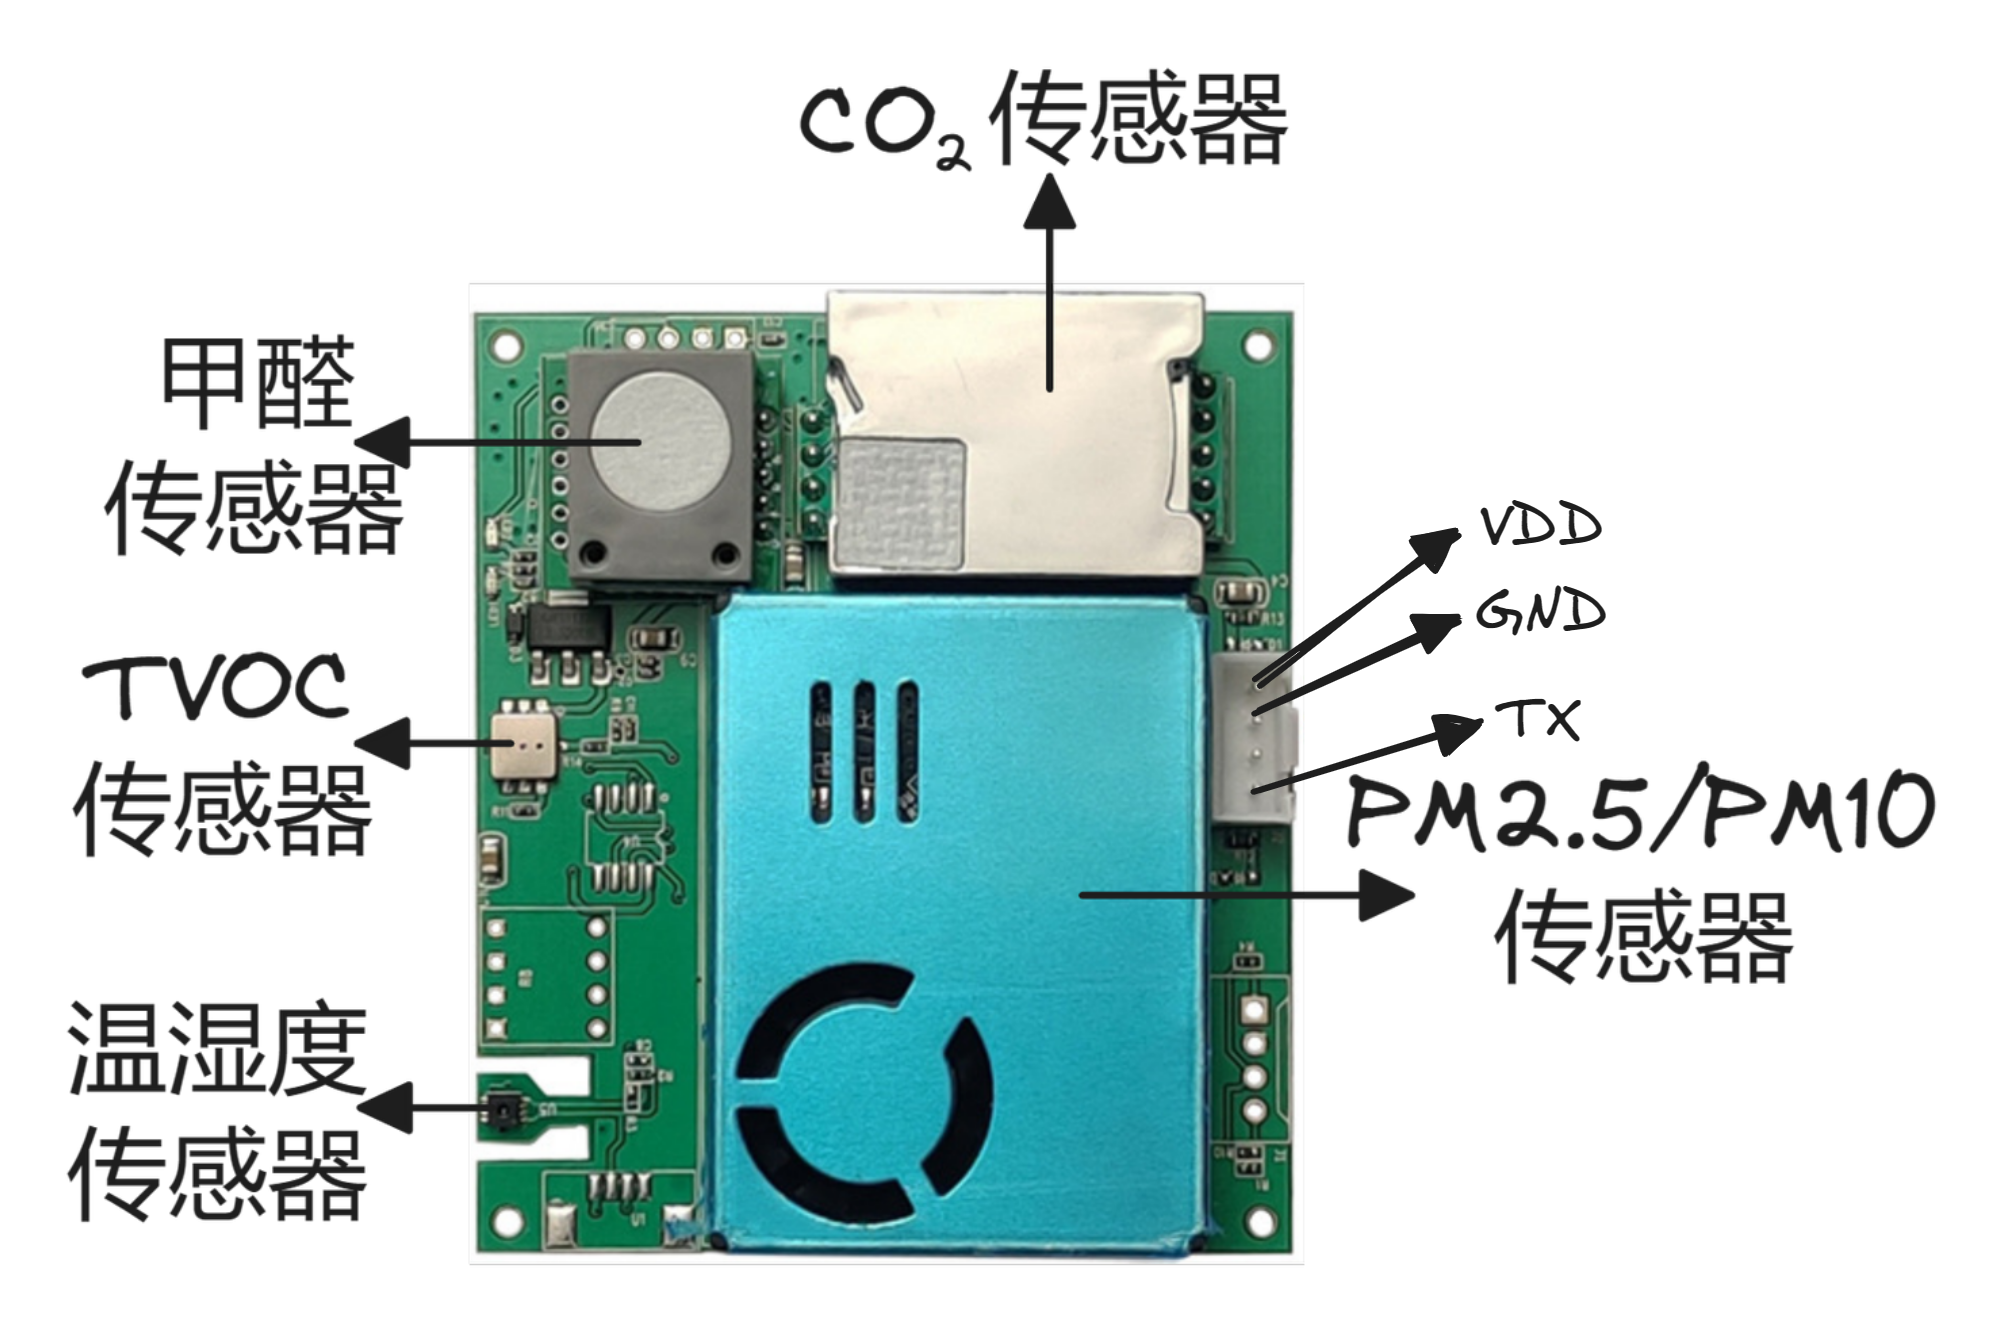
\includegraphics[width =.4\textwidth]{figures/sensor.png}
    \caption{传感器布局图}
    \label{sensor}
\end{wrapfigure}

本系统的设计方案传感器布局图如\autoref{sensor},原理框图如\autoref{block_diagram}所示,主要包括以下几个部分:

传感器模块:由 \ce{CO2} 、甲醛传感器、TVOC 传感器、PM2.5/PM10 传感器、温湿度传感器及信号调理电路
误差补偿及校正电路组成,负责采集空气质量的数据,并经过滤除干扰和误差校正后输出。

通信电路:由 MCU 和 A/D 转换器组成,负责对传感器模块输出的模拟信号进行数字化处理和软件误差修正,通过串口发送给嵌入式开发板。

嵌入式开发板:包含 RK3568、WIFI 模块、LVDS,负责对传感器输出的数字信号进行数据计算和逻辑控制,以及与其他模块进行通信。

数据显示模块:由 LCD 显示屏组成,负责显示实时的空气质量数值,以及报警提示,并提供一个交互界面用于修改报警阈值。

网页:由嵌入式开发板负责控制,提供一个远程显示实时的空气质量数值,以及报警提示,并提供一个交互界面用于修改报警阈值。

\begin{figure}[htbp]
    \centering
    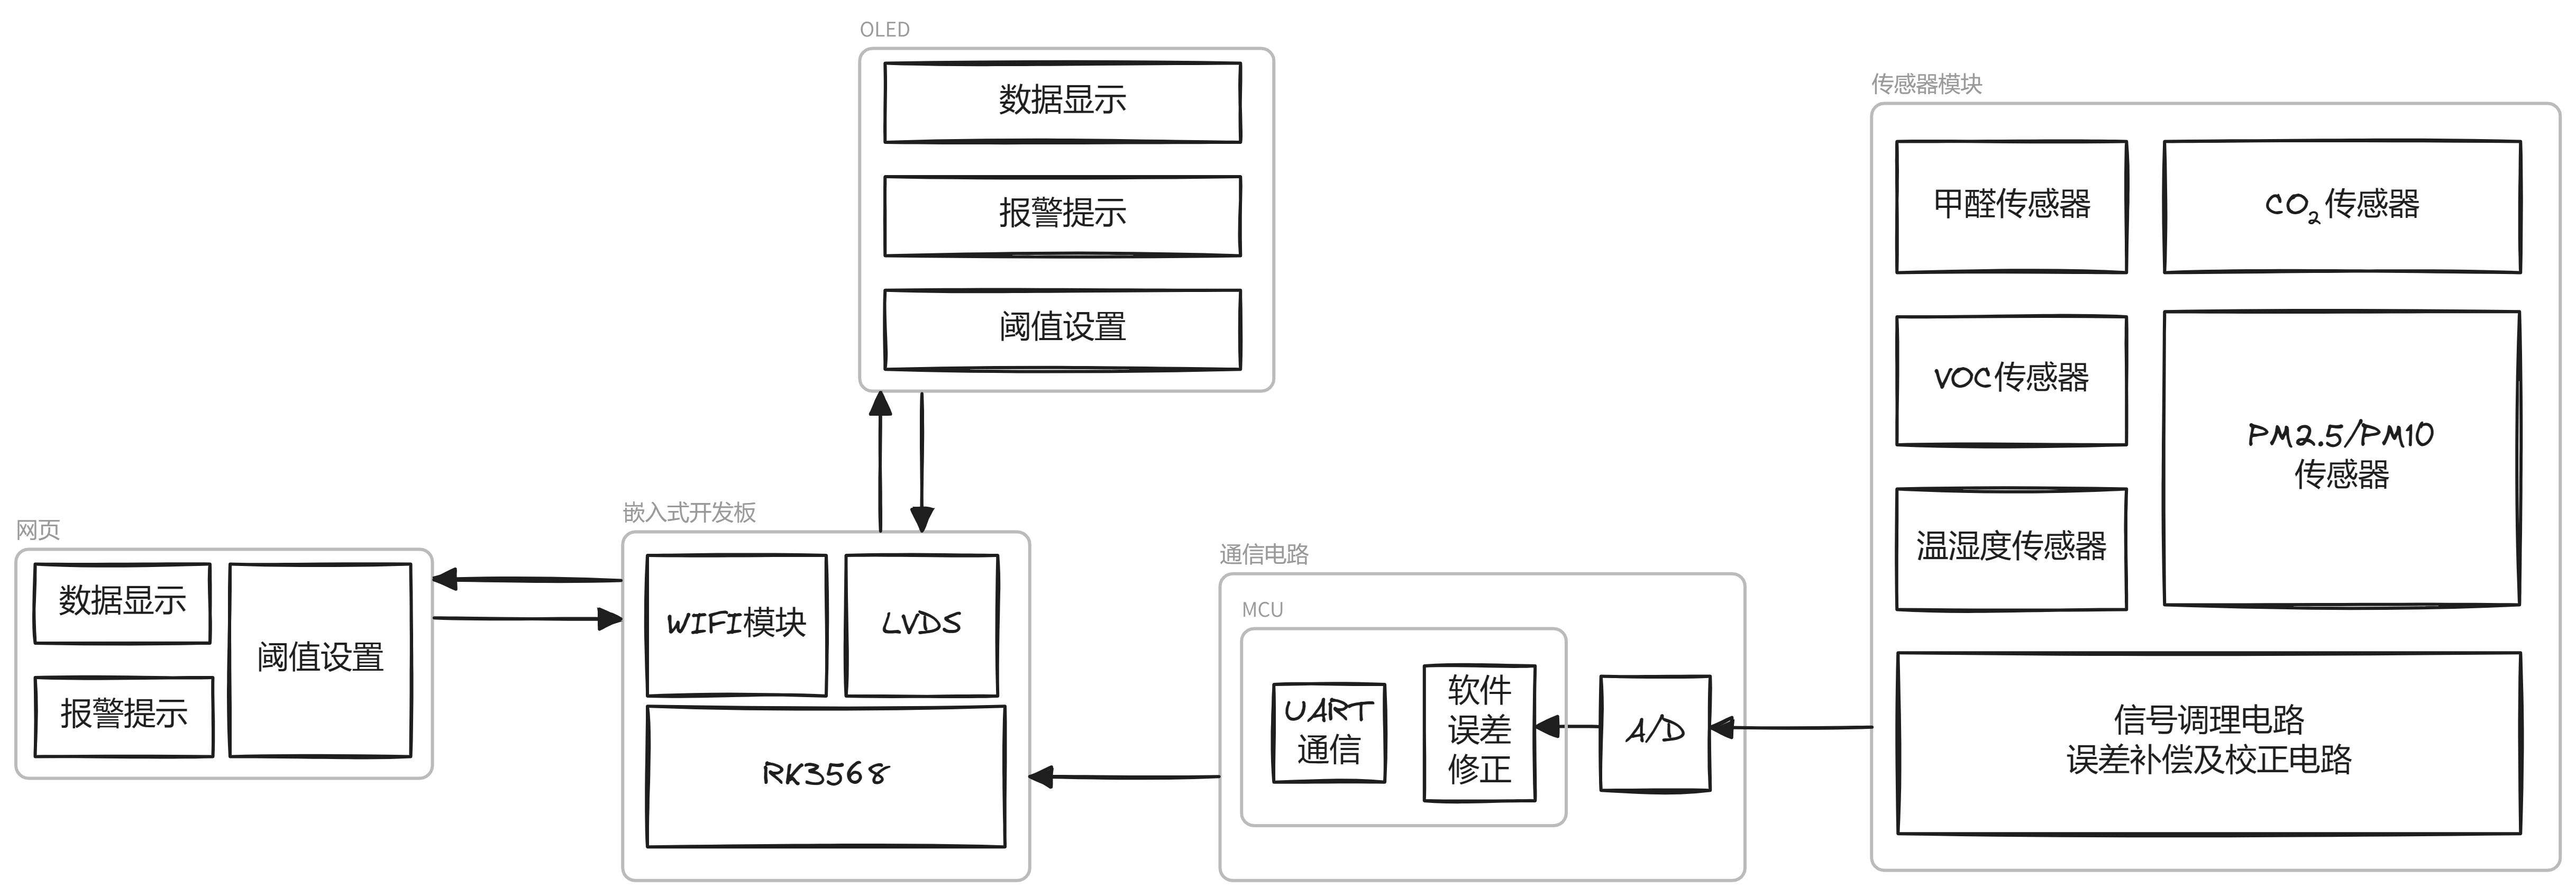
\includegraphics[width =.9\textwidth]{figures/block_diagram.png}
    \caption{原理框图}
    \label{block_diagram}
\end{figure}

\subsection{传感器模块设计原理} \label{sensor_design}
\subsubsection{\ce{CO2} 传感器}
红外非分散吸收(NDIR)气体传感器的工作原理是根据不同气体分子对于近
红外光谱的吸收特性,通过气体浓度与吸收强度关系如\autoref{Beer-Lambert Law},
分析计算并确定气体的浓度。\ce{CO2} 等由异种原子构成的分子在红外线波长区域具有吸收光谱,
\ce{CO2} 在 4200\unit{nm} 和 4320\unit{nm} 之间存在吸收峰值。
当对应某一气体特征吸收波长的光波通过被测气
体时,其强度将明显减弱,强度衰减程度与该气体浓度有关。
热电堆传感器由通常串联(或偶尔并联)的大量热电偶组成。
串联热电偶的输出电压取决于热电偶结与基准结之间的温度差。

在 NDIR 应用中,经过滤波的脉冲红外光施加于串联有源结点;因此,
结点加热,产生较小的热电电压。基准结点的温度由热敏电阻测量。
如果将红外光施加在双热电堆传感器上,并安装一对滤光器,
使其中一个滤光器中心波长在4260\unit{nm},而另一个中心波长在3910\unit{nm},
则通过测量两个热电堆的电压之比即可测得二氧化碳浓度。

\autoref{CO2_sensor}所示电路是一个基于 NDIR 原理的热电堆气体传感器完整电路。
该电路针对二氧化碳检测优化,但采用不同滤光器的热电堆之后亦可精确测量多种气体的浓度。

测量通道传感器的红外强度以指数关系递减,此关系称为朗伯-比尔定律:
\begin{equation}
    I = I_0 e^{-k l x}
    \label{Beer-Lambert Law}
\end{equation}
其中,$I$ 表示出射光强,$I_0$ 表示入射光强,$k$ 表示特定气体和滤光器组合的吸收系数。
$l$ 表示光源与检测器之间的等效光学路径长度,$x$ 表示气体浓度。

对于测量通道传感器输出,存在相应的输出电压变化 $V_0–V$:

\begin{equation}
    FA=\frac{V_0 - V}{V_0}=\frac{I_0 - I}{I_0}
    \label{FA}
\end{equation}
其中,$FA$ 表示相对吸收率,$V_0$ 表示入射光强对应传感器输出,$V$ 表示出射光强对应传感器输出。

将\autoref{Beer-Lambert Law}代入\autoref{FA},得到:
\begin{equation}
    FA=1-e^{-k l x}
\end{equation}

令 $b=kl$,并对传感器进行校准,校准的第一步要求对传感器组件施加低浓度的二氧化碳气体(或纯氮气,即$0\%$浓度的二氧化碳气体)。
校准的第二步要求将已知浓度($x_{CAL}$)的二氧化碳气体施加到组件上。

数据代入\autoref{Beer-Lambert Law}就可以写出含有两个未知数($I_0$ 和 $b$)的联立方程,从而求解出 $I_0$ 和 $b$ 的值。
然后,对于未知浓度($x$)的气体,联立已有方程可得\autoref{CO2},其中,$ACT$ 表示未知气体环境中测量通道传感器的峰峰值输出,
$REF$ 表示未知气体环境中基准通道传感器的峰峰值输出,$T$ 表示未知气体的温度,单位为 \unit{\kelvin}。

\begin{equation}
    x=\frac{T}{T_{LOW}}\left[\frac{\ln \left(\frac{ACT}{REF\times ZERO}\right)}{-b}\right]
    \label{CO2}
\end{equation}
系数 $\dfrac{T}{T_{LOW}}$ 补偿温度变化对气体浓度的影响(在此使用了理想气体定律)。

\subsubsection{甲醛传感器}
当气体通过扩散方式进入到传感器中时,测其化学性质 (如电流,电位,电量等)
的变化则可实现物质及含量的测定,传感器的正电极和负电极由一个电
解质液隔开,电化学传感器通过与被测气体发生反应并产生与气体浓度成正比的电信号来工作,
气体通过微小的透气孔与传感器产生反应,然后再经过透气
防水过滤膜,到达电极表面,气体与传感器电极发生反应,以产生充分的电信号,
同时防止电解质液出传感器,通过透气防水过滤膜扩散的气体与传感器电极
发生反应,传感的电极可以采用氧化反应和还原反应的机理,这些反应由针对备测气体
而设计的电极材料进行催化,通过电极间连接的电阻器,与被测气浓度
成正比的电流会在正电极与负电极之间流动,通过测量该电流的大小即可确定气体浓度。
其基本测量电路如\autoref{HCHO_sensor}所示。
该甲醛传感器检测甲醛时发生如下的电化学反应。

阳极:\ce{HCHO + H2O -> CO2 + 4H+ + 4e^-}

阴极:\ce{O2 + 4H+ + 4e^- -> 2H2O}

总反应式:\ce{HCHO + O2 -> CO2 + H2O}

\subsubsection{TVOC 传感器}
厚膜型气敏元件是将 \ce{SnO2} 和 \ce{ZnO} 等材料与硅凝胶混合制成能印刷的厚膜
胶,把厚膜胶用丝网印制到装有铂电极的氧化铝基片上,再经过烧结制成的气敏元件。
厚膜型气敏元件的工作原理是:当被测气体中的有害气体与厚膜胶接触时,
厚膜胶中的氧化物会与有害气体发生化学反应,使厚膜胶的电阻值发生变化,
通过测量电阻值的变化,可以得到有害气体的浓度。
其基本测量电路如\autoref{TVOC_sensor}所示。

输出电压的大小可表示为:
\begin{equation}
    U_{out} = I_oR_L = \frac{U_i}{R_s + R_L}
\end{equation}
其中,$R_L$ 表示负载电阻(兼作取样电阻),$R_s$ 表示气敏电阻测试支路的电阻。

由上式可知,当 $R_s$ 增大时,$U_{out}$ 减小,反之亦然。
因此,通过测量输出电压即可测得气敏元件的电阻值 $R_s$,从而得到被测气体的浓度。

\subsubsection{PM2.5/PM10 传感器}
PM2.5/PM10 传感器采用激光散射原理,当空气颗粒进入激光区域时,会发生光散射。
特定方向的光散射信号与颗粒直径有关。通过使用光电检测器(光电二极管),
由于光电效应,如\autoref{photoelectric}所示,会产生电流信号。当电流信号经过电路放大和处理后,
在一个采样时间周期内,可以将不同颗粒大小的质量浓度转换为最终的 PM2.5 和 PM10 质量浓度。
测量示意图如\autoref{PM_sensor}所示。


\begin{equation}
    E_k = \frac{1}{2} mv^2 = h\omega - A_0
    \label{photoelectric}
\end{equation}
其中,$m$ 表示电子的质量,$v$ 表示电子逸出的初始速度,$h$ 表示普朗克常数。

\subsubsection{湿度传感器}
高分子式电阻湿度传感器是利用高分子电解质吸湿而导致电阻率发生变化的基本原理来进行测量的,
通常将含有强极性基的高分子电解质及其盐类,例如\ce{-NH_4^+CI^-}、\ce{-NH2}、\ce{-SO_3^-H^+},
等高分子材料制成感湿电阻膜。当水吸附在强极性基高分子上时,随着湿度的增加吸附量增大,
吸附水分子凝聚成液态。在低湿吸附量少的情况下,由于没有荷电离子产生,电阻值很高;
当相对湿度增加时,凝聚化的吸附水就成为导电通道,高分子电解质的成对离子主要起载流子作用。
此外,由吸附水自身离解出来的质子(\ce{H+})及水和氢离子(\ce{H3O+}) 也起电荷载流子作用,这就使得载流子数目急剧增加,
传感器的电阻急剧下降。利用高分子电解质在不同湿度条件下电离产生的导电离子数量不等使阻值发生变化,就可以测定环境中的湿度。
其基本测量电路如\autoref{Humidity_sensor}所示。


\section{电路原理图}
\subsection{传感器模块电路原理图}
各个传感器模块的电路原理图如下所示,由于篇幅所限,每个模块的电路原理图已包含测量电路部分,误差补偿部分,
不再单独给出。其中 $U_o$ 通过 ADC 转换为数字信号,经过嵌入式开发板处理后,通过 LCD 显示出来。
\begin{figure}[htbp]
    \centering
    \begin{minipage}{0.6\textwidth}
        \centering
        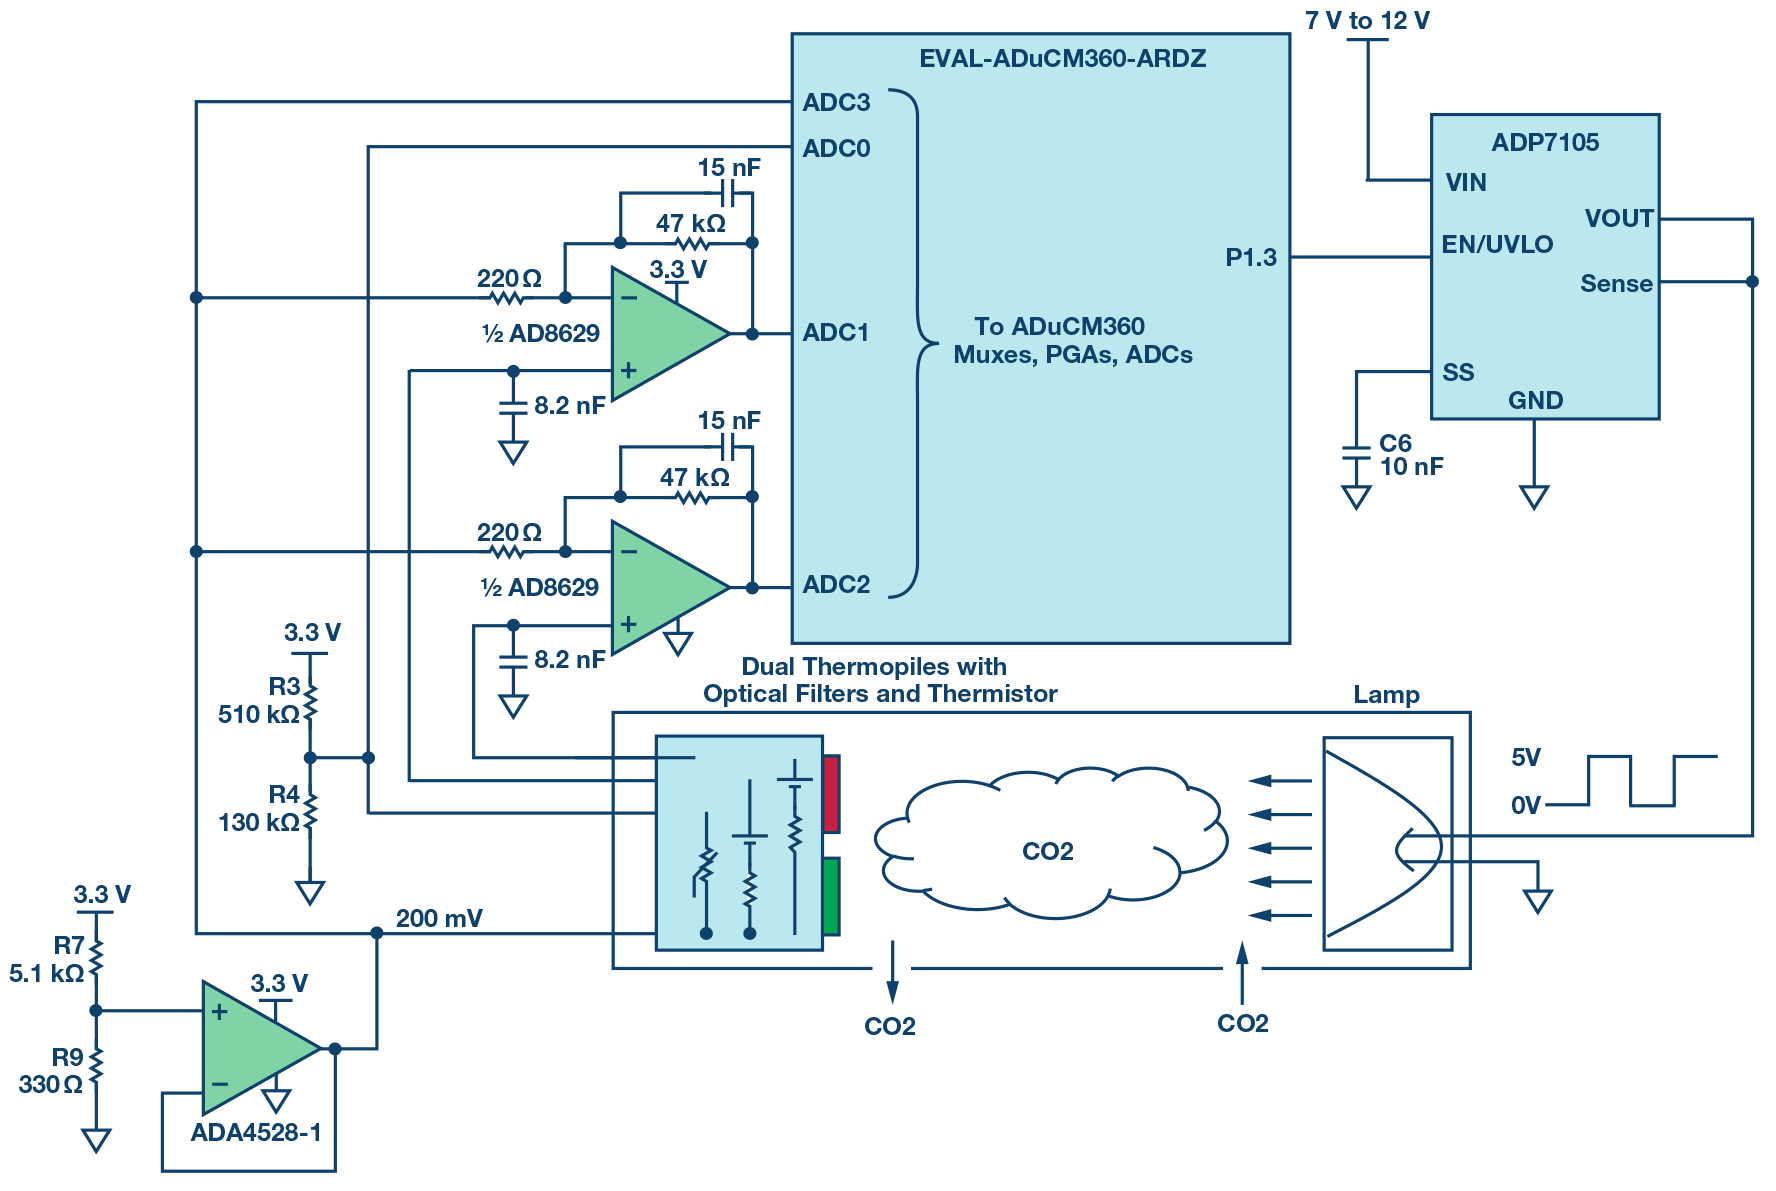
\includegraphics[width =1\textwidth]{figures/CO2_sensor.png}
        \caption{NDIR 气体检测电路}
        \label{CO2_sensor}
    \end{minipage}
    \begin{minipage}{0.35\textwidth}
        \centering
        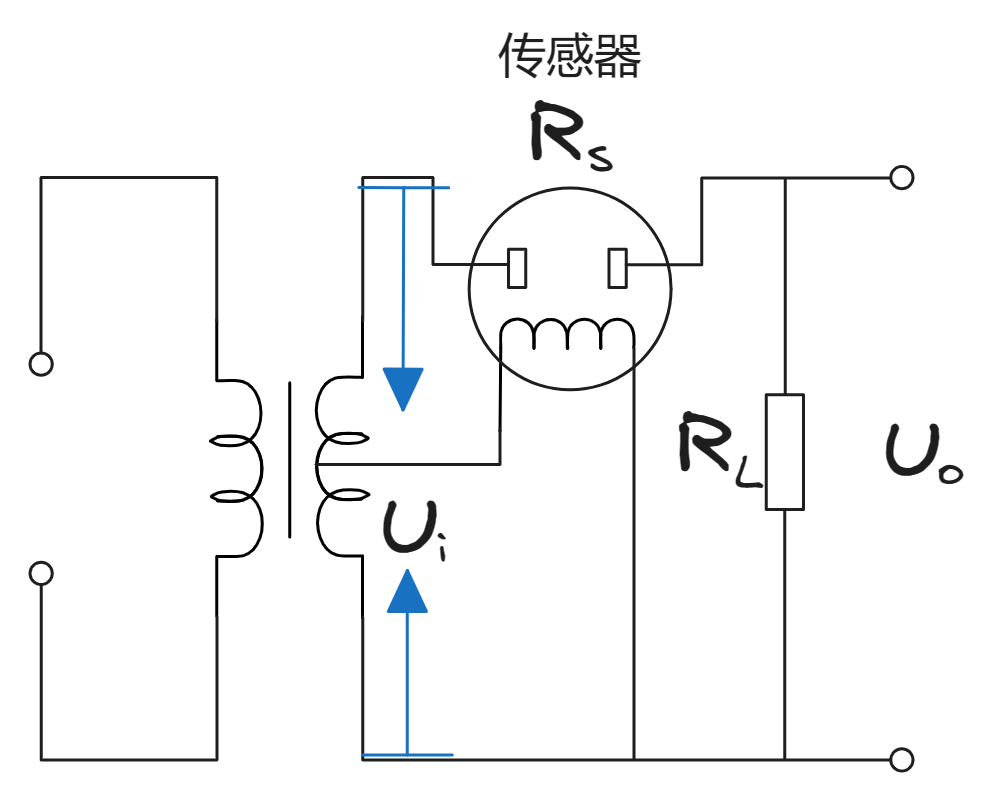
\includegraphics[width =.7\textwidth]{figures/TVOC_sensor.png}
        \caption{TVOC 气体检测电路}
        \label{TVOC_sensor}
    \end{minipage}
\end{figure}

\begin{figure}[htbp]
    \centering
    \begin{minipage}{0.45\textwidth}
        \centering
        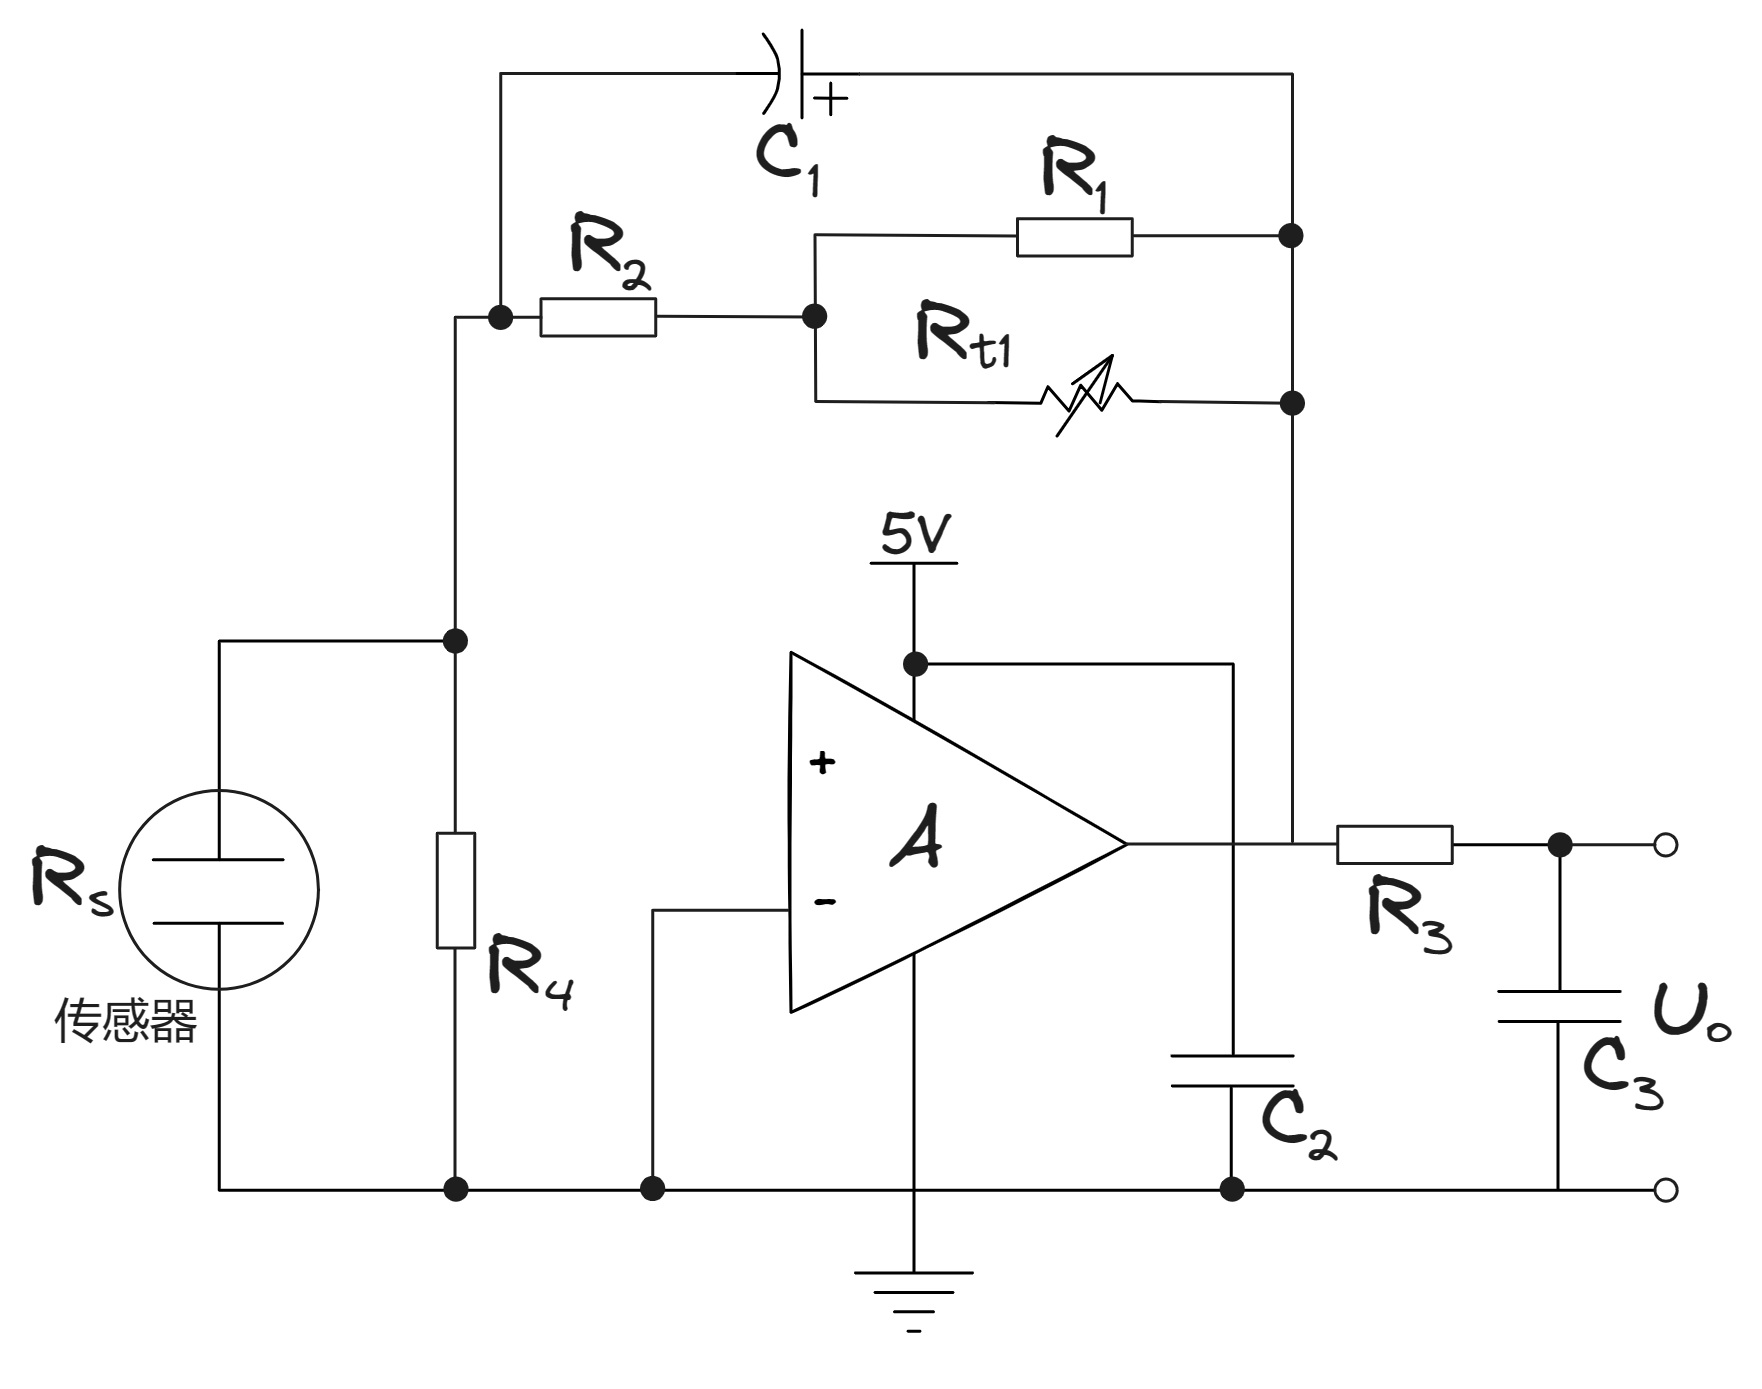
\includegraphics[width =.8\textwidth]{figures/HCHO_sensor.png}
        \caption{甲醛气体检测电路}
        \label{HCHO_sensor}
    \end{minipage}
    \begin{minipage}{0.45\textwidth}
        \centering
        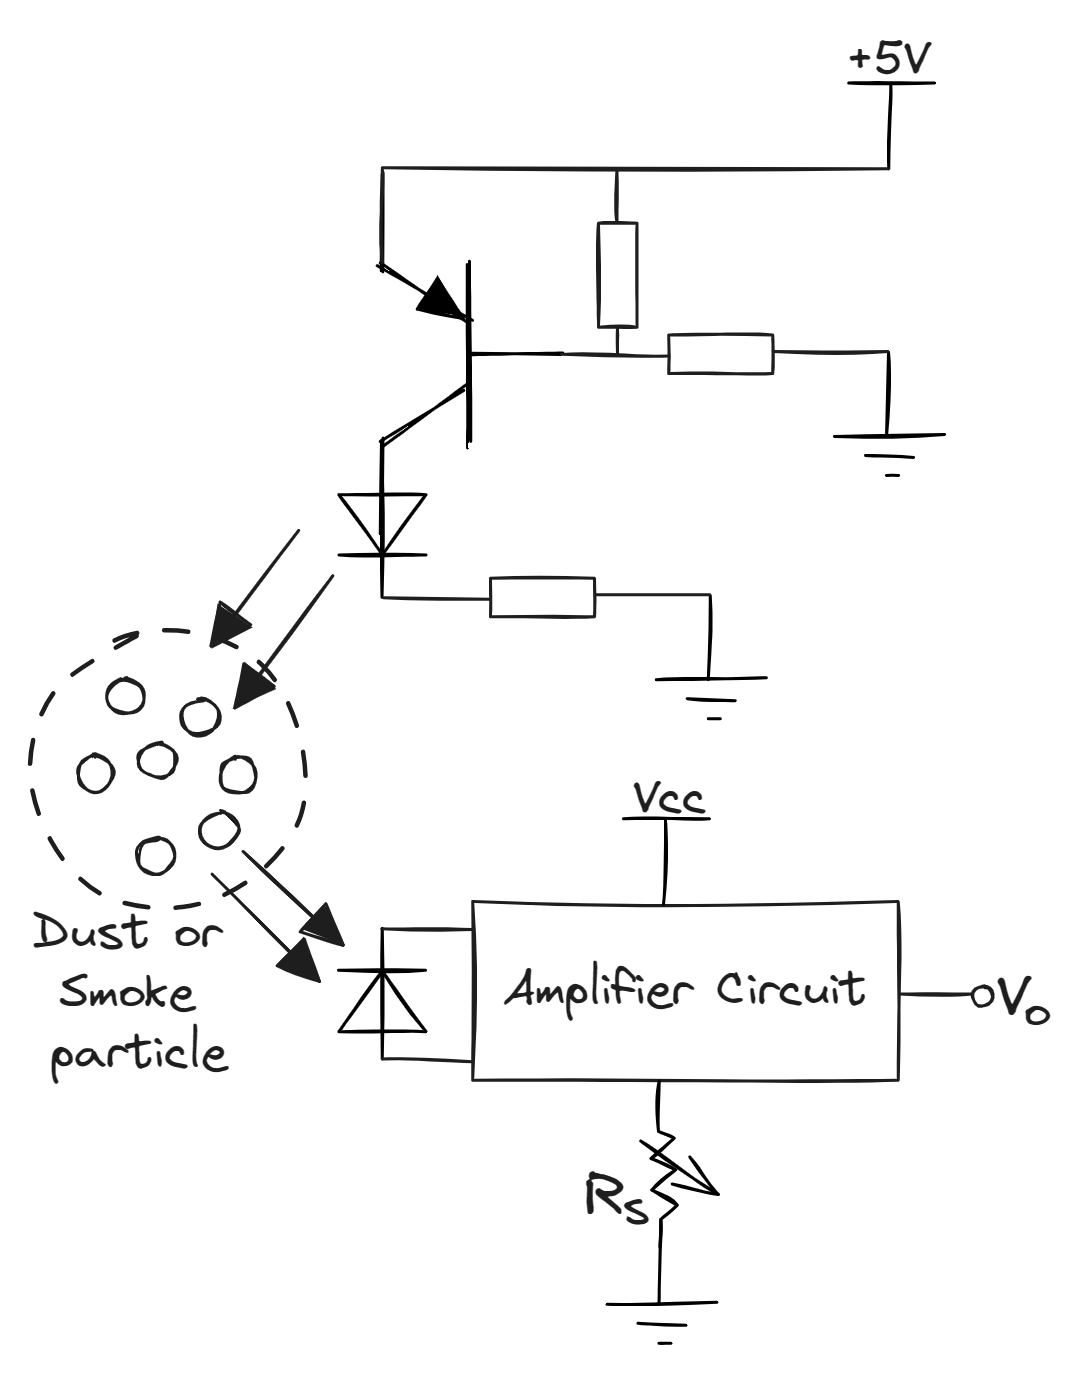
\includegraphics[width =.75\textwidth]{figures/PM_sensor.png}
        \caption{PM2.5/PM10 气体检测示意图}
        \label{PM_sensor}
    \end{minipage}
\end{figure}

\begin{figure}[htbp]
    \centering
    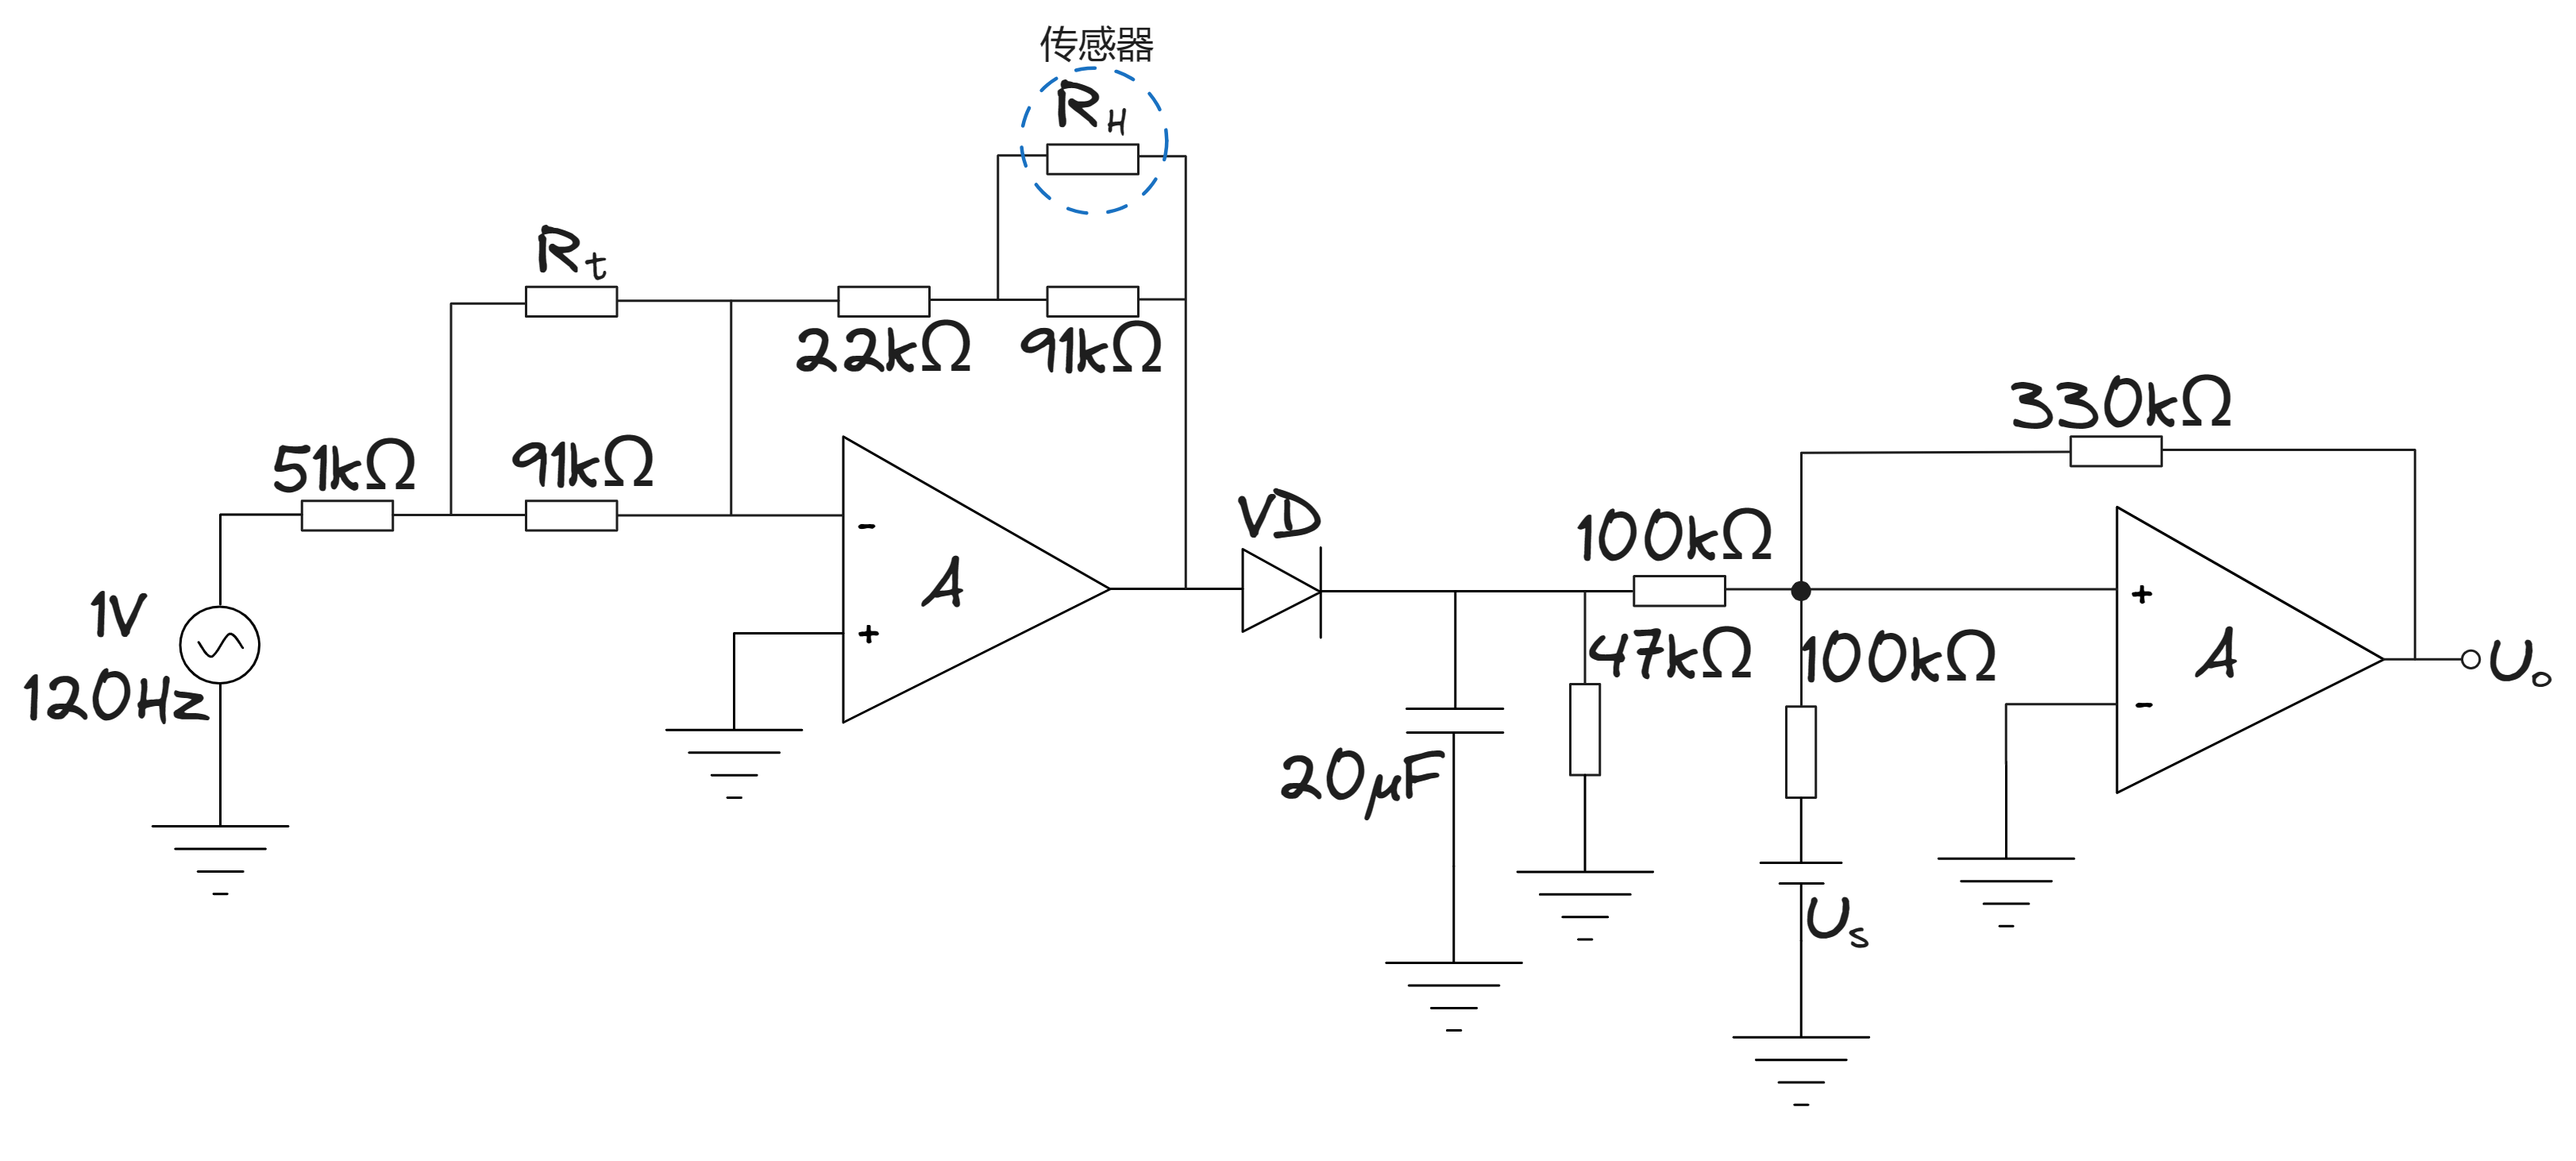
\includegraphics[width =.8\textwidth]{figures/Humidity_sensor.png}
    \caption{湿度测量电路}
    \label{Humidity_sensor}
\end{figure}

\subsection{通信电路原理图}
通信电路原理图如\autoref{communication}所示,其中 $U_o$ 通过 ADC 转换为数字信号,经过 MCU 处理后,通过串口传输给 RK3568 开发板。
\begin{figure}[htbp]
    \centering
    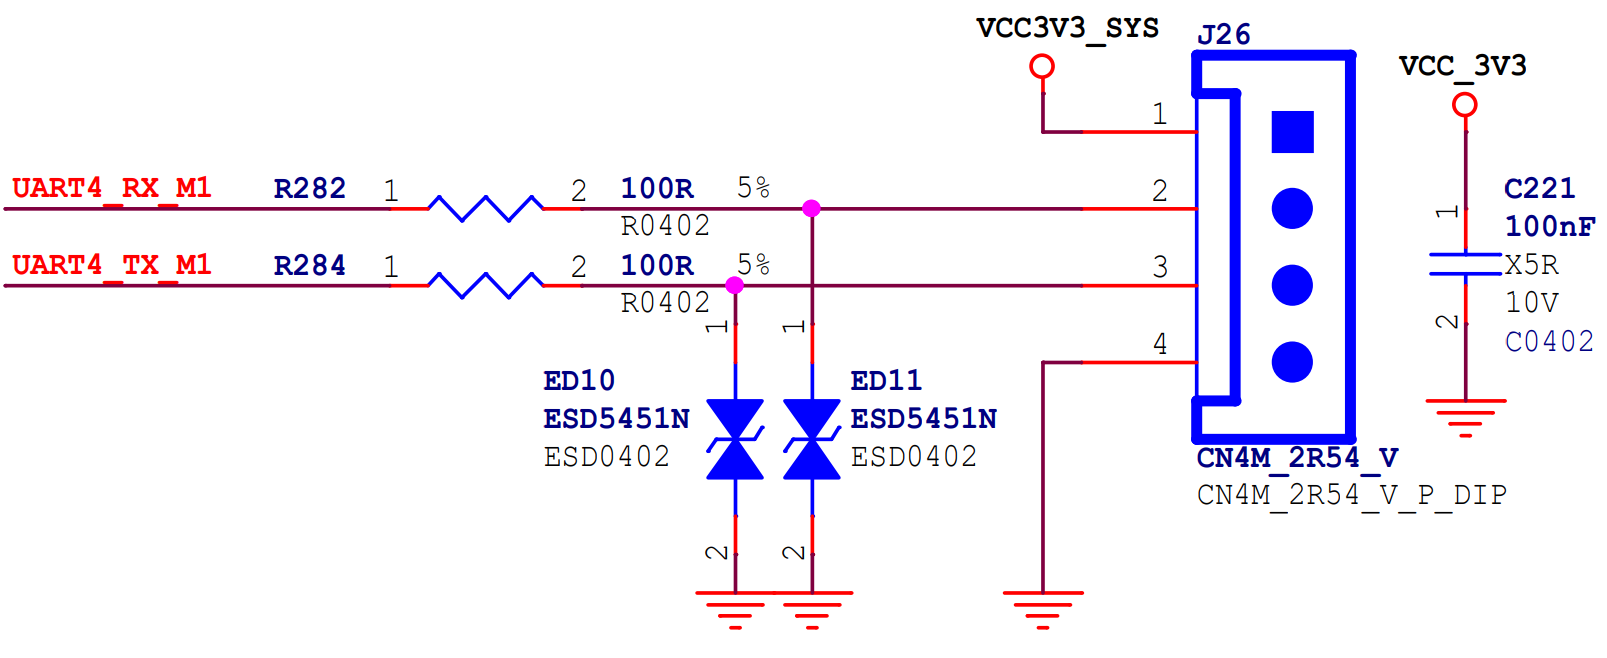
\includegraphics[width =.6\textwidth]{figures/UART.png}
    \caption{通信电路原理图}
    \label{communication}
\end{figure}

\subsection{WIFI 模块电路原理图}
WIFI 模块电路原理图如\autoref{WIFI}所示,用于 RK3568 开发板连接网络,为其提供进行网页前后端交互处理的支持。
\begin{figure}[htbp]
    \centering
    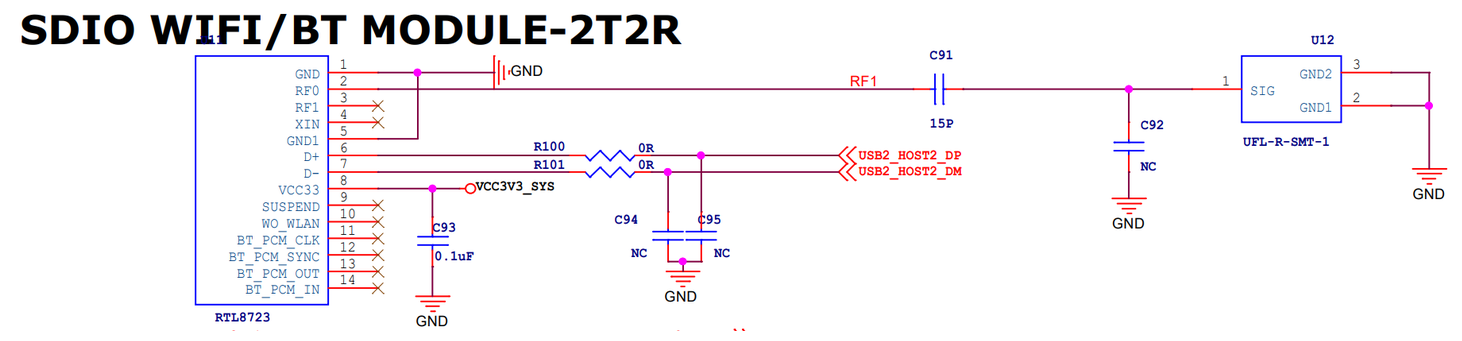
\includegraphics[width =1\textwidth]{figures/WIFI.png}
    \caption{WIFI 模块电路原理图}
    \label{WIFI}
\end{figure}

\subsection{USB 电路原理图}
USB 电路原理图如\autoref{USB}所示,用于 RK3568 开发板连接键盘、鼠标等外设,为其提供进行人机交互处理的支持。
\begin{figure}[htbp]
    \centering
    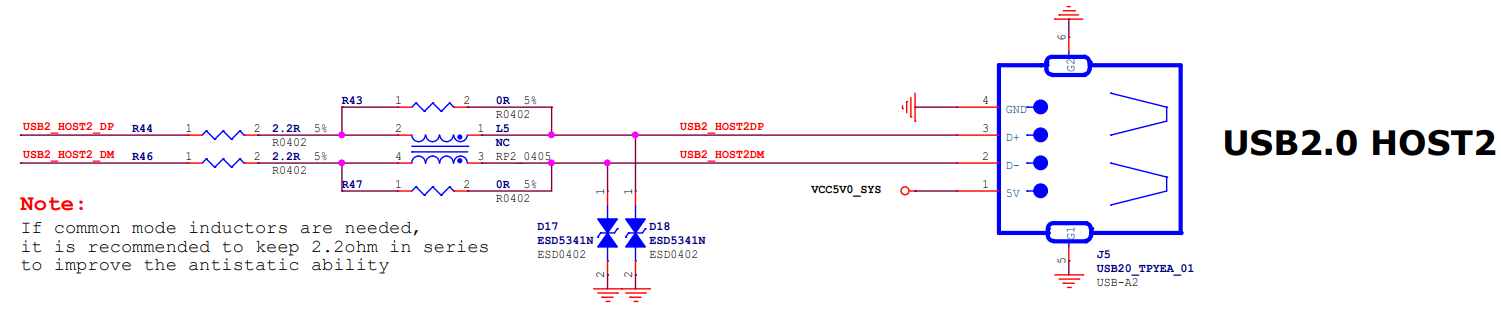
\includegraphics[width =.9\textwidth]{figures/USB.png}
    \caption{USB 电路原理图}
    \label{USB}
\end{figure}

\subsection{LVDS 电路原理图}
LVDS 电路原理图如\autoref{LVDS}所示,用于 RK3568 开发板连接 LCD 显示屏,为其提供进行数据显示的支持。
\begin{figure}[htbp]
    \centering
    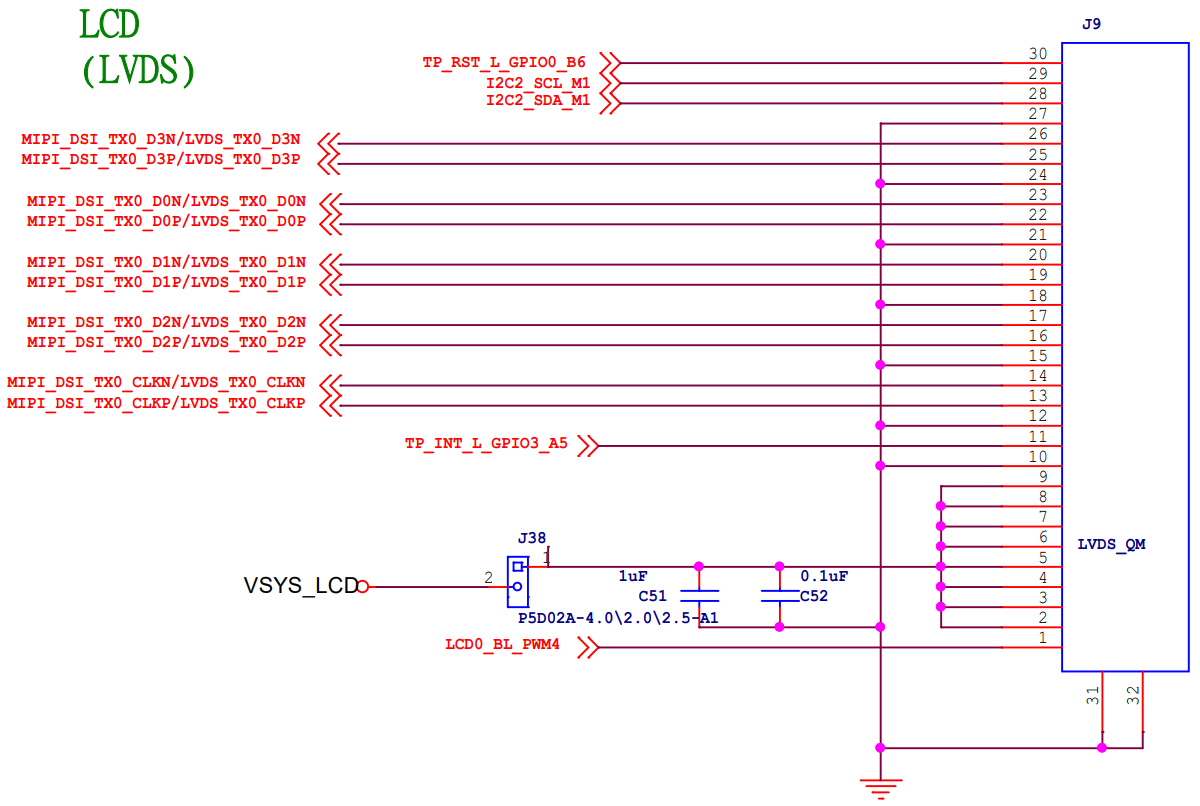
\includegraphics[width =.8\textwidth]{figures/LCD.png}
    \caption{LVDS 电路原理图}
    \label{LVDS}
\end{figure}

\subsection{电源电路原理图}
电源电路原理图如\autoref{power}所示,用于为各个模块提供电源。
\begin{figure}[htbp]
    \centering
    \includegraphics[width =1\textwidth]{figures/power.png}
    \caption{电源电路原理图}
    \label{power}
\end{figure}

\newpage
\section{软件流程及算法}
\subsection{软件流程}
软件流程如\autoref{software_flow}所示,主要包括以下几个部分:
\begin{enumerate}
    \item 初始化:初始化各个传感器以及其他外设
    \item 读取传感器数据:读取各个传感器的数据,通过 ADC 转换为数字信号
    \item 数据处理:对传感器数据进行处理,包括误差补偿,校正,单位转换等
    \item 显示数据:将处理后的数据显示在 LCD 屏幕上
    \item 读取报警阈值:读取用户设置的报警阈值
    \item 报警:根据读取的报警阈值,判断是否报警
    \item 上传数据:将数据上传到网页
    \item 循环:循环执行以上步骤
\end{enumerate}

\begin{figure}[htbp]
    \centering
    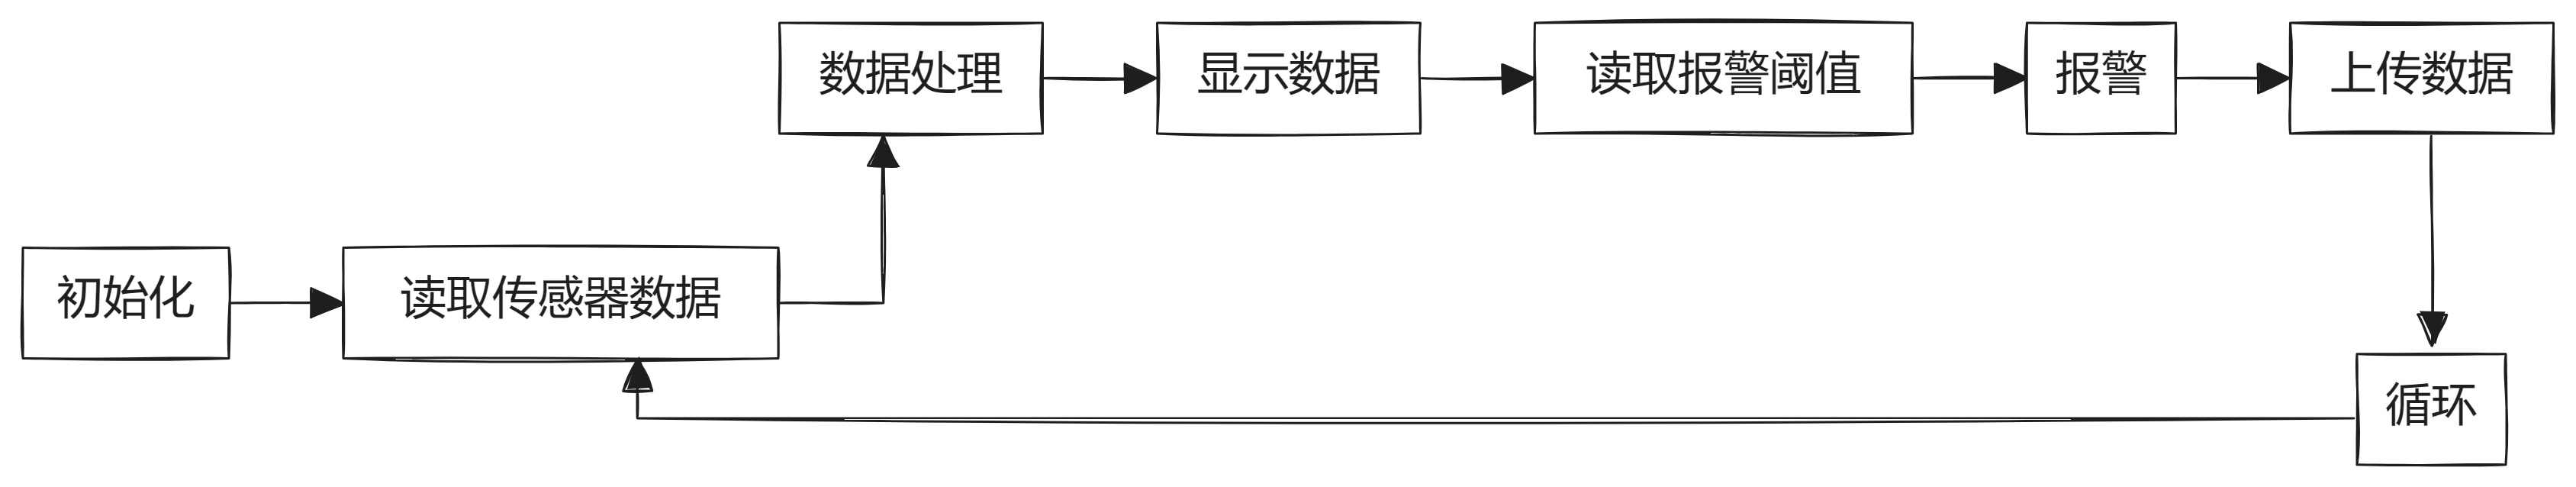
\includegraphics[width =.8\textwidth]{figures/software_flow.png}
    \caption{软件流程}
    \label{software_flow}
\end{figure}

\subsection{算法}
\subsubsection{传感器数据处理}
传感器数据获取由 MCU 处理,采用 \texttt{C} 语言编写,通过读取 ADC 的引脚电压,并将其转换为数字量。

ADC 代码如下:
\begin{lstlisting}[style=Cstyle]
    double getADC(ADC_HandleTypeDef *pin)
    {
        unsigned int adc;
        HAL_ADC_Start (pin);
        adc = HAL_ADC_GetValue(pin);
        return adc; 
    }
\end{lstlisting}
\newpage
误差补偿公式已于\autoref{sensor_design}给出,由于篇幅所限,
各个传感器模块所测电压与气体浓度的关系见对应传感器的数据手册,
此处仅给出传感器数据处理算法。

电压量转化为气体浓度的代码如下:
\begin{lstlisting}[style=Cstyle]
    void ADC_proc(void)
    {
      for (uint8_t t = 0; t < 20; t++)
      {
        HAL_GPIO_WritePin(GPIOA, GPIO_PIN_2, GPIO_PIN_RESET);
        delay_us(320);
        HAL_GPIO_WritePin(GPIOA, GPIO_PIN_2, GPIO_PIN_SET);
        delay_us(280);
        adc_temp = getADC(&hadc1);
        delay_ms(9);
        delay_us(400);
        adc_sum = adc_sum + adc_temp;
      }
      adc_sum = adc_sum / 20;//`\scriptsize\color{green!40!black}{多次采集取平均值}`
    
      voltage = adc_sum * 0.806;//`\scriptsize\color{green!40!black}{需要换算后得到实际数值}`
    
      result = (unsigned int)(0.18 * voltage);//`\scriptsize\color{green!40!black}{电压转换为浓度}`
    }
\end{lstlisting}

通过电压——浓度曲线线性部分的关系,如\autoref{voltage_concentration}所示,
将电压量转化为气体浓度,再通过误差补偿公式计算修正,得到传感器的数据。
\begin{figure}[htbp]
    \centering
\begin{tikzpicture}
    \draw[->] (-0.2,0) --(6,0) node[right] {浓度(\unit{\ug /m^3})};
    \draw[->] (0,-0.2) --(0,6) node[above] {电压($V$)};
    \draw[domain =0:4] plot (\x ,{0.1* exp(\x)});
    \draw[dashed] (3, 0.76) -- (4, 5.35);
\end{tikzpicture}
    \caption{电压——浓度曲线示意图}
    \label{voltage_concentration}
\end{figure}

\newpage
\subsubsection{显示数据}
传感器数据经 MCU 处理后经由串口将数据传输给 RK3568 开发板,它通过 LVDS 协议驱动 LCD 显示屏显示数据。
相关程序采用 \texttt{Python} 语言编写。

读取串口数据的代码如下:
\begin{lstlisting}[style=Pythonstyle,name=serial_read.py]
    import serial

    # Initialize serial port
    ser = serial.Serial('/dev/ttyS4', 9600, timeout=1)
    
    # Initialize thresholds
    thresholds = {'eCO2': 4000, 'eCH2O': 15, 'TVOC': 20, 'PM2.5': 50, 'PM10': 70, 'Temperature': 25, 'Humidity': 35}
    
    def read_m701_data(serial_port):
        # Read response
        response = serial_port.read(17)
    
        # Check if the response has the expected length
        if len(response) != 17:
            print("Invalid response length")
            return None
    
        # Verify frame header
        if response[0] != 0x3C or response[1] != 0x02:
            print("Invalid frame header")
            return None
    
        # Parse response
        data = {'eCO2': int.from_bytes(response[2:4], byteorder='big'),
                'eCH2O': int.from_bytes(response[4:6], byteorder='big'),
                'TVOC': int.from_bytes(response[6:8], byteorder='big'),
                'PM2.5': int.from_bytes(response[8:10], byteorder='big'),
                'PM10': int.from_bytes(response[10:12], byteorder='big'), 
                'Temperature': response[12] + response[13] / 10,
                'Humidity': response[14] + response[15] / 10}
\end{lstlisting}
\newpage
\begin{lstlisting}[style=Pythonstyle,name=serial_read.py]
        # Verify checksum
        checksum = sum(response[:-1]) & 0xFF
        if checksum != response[-1]:
            print("Invalid checksum")
            return None
    
        return data
\end{lstlisting}

显示空气质量数据及报警提示的代码如下:

\begin{lstlisting}[style=Pythonstyle,name=display_data.py]
    import curses
    
    def display_data(stdscr, data):
    warnings = []
    stdscr.clear()
    # Check if data is valid
    if data is None:
        stdscr.clear()
        stdscr.addstr(0, 0, "`\color{teal!70!white}{数据读取中...}`")
        stdscr.refresh()
        return
    # Display data
    stdscr.addstr(0, 0, "`\color{teal!70!white}{CO2含量:}` {} ppm".format(data['eCO2']))
    stdscr.addstr(1, 0, "`\color{teal!70!white}{CH2O含量:}` {} ug/m3".format(data['eCH2O']))
    stdscr.addstr(2, 0, "`\color{teal!70!white}{TVOC含量:}` {} ug/m3".format(data['TVOC']))
    stdscr.addstr(3, 0, "`\color{teal!70!white}{PM2.5含量:}` {} ug/m3".format(data['PM2.5']))
    stdscr.addstr(4, 0, "`\color{teal!70!white}{PM10含量:}` {} ug/m3".format(data['PM10']))
    stdscr.addstr(5, 0, "`\color{teal!70!white}{温度:}` {} `\color{teal!70!white}℃`".format(data['Temperature']))
    stdscr.addstr(6, 0, "`\color{teal!70!white}{湿度:}` {} %".format(data['Humidity']))
    # Check if data is exceeding thresholds
    for i, (key, value) in enumerate(data.items()):
        if value > thresholds[key]:
            warnings.append(key)
    if len(warnings) > 0:
            stdscr.addstr(7, 0, f'`\color{teal!70!white}{警告:}`{", ".join(warnings)}`\color{teal!70!white}{超过阈值}`')
    else:
        stdscr.addstr(7, 0, '`\color{teal!70!white}{空气指标正常}`')
    stdscr.refresh()

\end{lstlisting}

\subsubsection{读取报警阈值}
报警阈值通过键盘输入,程序采用非阻塞读取按键是否按下,以免干扰传感器数据的读取。
当检测到按键 \texttt{I} 按下时,进入阈值设置模式,上下键用于选择要设置的阈值,回车为确认键,
数字键用于填写阈值,\texttt{ESC} 键用于退出阈值设置模式。

设置报警阈值的代码如下:

\begin{lstlisting}[style=Pythonstyle, name=handle_input.py]
    def handle_input(stdscr, data):
    stdscr.nodelay(True)  # Enable non-blocking mode
    c = stdscr.getch()
    stdscr.nodelay(False)  # Restore blocking mode
    if c == ord('i'):
        # Enter threshold setting mode
        selected = 0
        while True:
            stdscr.clear()
            for i, key in enumerate(data.keys()):
                if i == selected:
                    stdscr.addstr(i, 0, "{}: {} ".format(key, data[key]), curses.A_REVERSE)
                else:
                    stdscr.addstr(i, 0, "{}: {} ".format(key, data[key]))
            stdscr.addstr(7, 0, "`\color{teal!70!white}{按上下键选择阈值,按回车确认}`")
            stdscr.refresh()
            c = stdscr.getch()
            if c == curses.KEY_UP:
                selected = (selected - 1) % len(data)
            elif c == curses.KEY_DOWN:
                selected = (selected + 1) % len(data)
            elif c == curses.KEY_ENTER or c == 10 or c == 13:
                for key in data.keys():
                    if key == list(data.keys())[selected]:
                        stdscr.addstr(8, 0, "{} `\color{teal!70!white}{阈值:}` ".format(key))
                        stdscr.refresh()
                        threshold = ''
                        while True:
                            c = stdscr.getch()
                            if c == curses.KEY_ENTER or c == 10 or c == 13:
\end{lstlisting}
\newpage
\begin{lstlisting}[style=Pythonstyle, name=handle_input.py]
                                if len(threshold) <= 4:
                                    thresholds[key] = int(threshold)
                                    break
                            elif c >= ord('0') and c <= ord('9'):
                                if len(threshold) < 4:
                                    threshold += chr(c)
                                    stdscr.addstr(8, len("{} `\color{teal!70!white}{阈值:}` "\
                                    .format(key)) + len(threshold), chr(c))
                                    stdscr.refresh()
                            elif c == 27:  # esc
                                break
                break
            elif c == 27:  # esc
                break
\end{lstlisting}

\subsubsection{主函数}
主函数如下所示:
\begin{lstlisting}[style=Pythonstyle, name=main.py]
    def main(stdscr):
    while True:
        data = read_m701_data(ser)
        display_data(stdscr, data)
        handle_input(stdscr, thresholds)
        curses.napms(100)  # Delay 100ms

if __name__ == '__main__':
    curses.wrapper(main)
\end{lstlisting}

\subsubsection{网页相关}
网页后端采用 \texttt{Flask} 框架,前端采用 \texttt{HTML+CSS+JS} 编写,后端主要实现了以下几个功能:
向前端传输空气质量数据以及报警信息,接收前端表单数据,修改报警阈值。
前端主要实现了以下几个功能:显示空气质量数据以及报警信息,修改报警阈值。
同时,前端还实现了自动更新数据的功能。另外为了避免接收传感器数据时阻塞网页的运行,
采用了多线程的方式,将数据读取和网页运行分开。

后端代码如下所示:
\newpage
\begin{lstlisting}[style=Pythonstyle, name=app.py]
    from flask import Flask, render_template, request, jsonify
    import threading

    app = Flask(__name__)
    def read_data():
        serial_port = serial.Serial('/dev/ttyS4', 9600, timeout=1)
        while True:
            global data
            data = read_m701_data(serial_port)

    @app.route('/data', methods=['GET'])
    def get_data():
        global data, warnings
        return jsonify(data=data, warnings=warnings)

    @app.route('/', methods=['GET', 'POST'])
    def home():
        global thresholds, warnings
        if request.method == 'POST':
            # Update thresholds
            for key in thresholds.keys():
                thresholds[key] = float(request.form[key])
        # Get warnings
        warnings = {key: value > thresholds[key] for key, value in data.items()}
        return render_template('home.html', data=data, warnings=warnings, thresholds=thresholds)

    if __name__ == '__main__':
        # Start a new thread for data reading
        threading.Thread(target=read_data).start()
        app.run(host='0.0.0.0', port=5000, debug=True)
\end{lstlisting}

前端代码如下所示:
\begin{lstlisting}[style=htmlstyle, name=home.html, title={home.html}]
    <!DOCTYPE html>
    <html>
    <head>
\end{lstlisting}
\newpage
\begin{lstlisting}[style=htmlstyle, name=home.html]
        <title>Monitor</title>
        <meta charset="UTF-8">
        <script src=
        "https://ajax.aspnetcdn.com/ajax/jQuery/jquery-3.5.1.min.js"></script>
        <script src="updateTable.js"></script>
    </head>
    <body>
        <table>
            
            <tr>
                <td>{{ key }}</td>
                <td>{{ value }}</td>
                <td>{{ 'Warning' if warnings[key] else '' }}</td>
            </tr>
            
        </table>
        <p>`设置阈值`</p>
        <form method="POST">
            
            <div>
                <label for="{{ key }}">{{ key }}</label>
                <input type="text" id="{{ key }}" name=
                "{{ key }}" value="{{ value }}">
            </div>
            
            <input type="submit" value="`\color{teal!70!white}{更新}`">
        </form>
    </body>
    </html>
\end{lstlisting}

\begin{lstlisting}[style=jsstyle, name=updateTable.js, title={updateTable.js}]
    function updateTable() {
        $.ajax({
            url: '/data', 
            type: 'GET',
            success: function(receivedData) {
                var data = receivedData.data;
                var warnings = receivedData.warnings;
\end{lstlisting}
\begin{lstlisting}[style=jsstyle, name=updateTable.js]
                $('table').empty();
                $.each(data, function(key, value) {
                    $('table').append('<tr><td>' + key + '</td><td>' + value + '</td><td>' + (warnings[key] ? 'Warning' : '') + '</td></tr>');
                });
            }
        });
    }

    setInterval(updateTable, 1000);
\end{lstlisting}

\section{特性指标标定方案}
\subsection{灵敏度}
灵敏度是气敏元件的一个重要参数,它标志着气敏元件对气体的敏感程度。
用阻值变化量 $\Delta R$ 与气体浓度变化量 $\Delta P$ 的比值来表示。即
\begin{equation}
    S = \frac{\Delta R}{\Delta P}
\end{equation}
灵敏度还有另一种表示方法,即气敏元件在空气中的阻值 $R_0$ 与在被测气体中的阻值 $R$ 的比值,即
\begin{equation}
    K = \frac{R_0}{R}
\end{equation}
\subsection{响应时间}
从气敏元件接触到一定浓度的被测气体开始,
至气敏元件的阻值达到该浓度下新的恒定值所需要的时间称为响应时间。
它表示气敏元件对被测气体浓度的响应速度。
\subsection{选择性}
指在多种气体共存的条件下,气敏元件区分气体种类的能力。
对某种气体选择性好,表明气敏元件对其灵敏度较高。选择性是气敏元件的重要特性。
\subsection{稳定性}
当被测气体浓度不变时,若其他条件(如温度、压力、 磁场等)发生改变,
在规定的时同内气敏元件输出特性保持不变的能力,称为稳定性。
稳定性反映了气敏元件的抗干扰能力。
\subsection{温度特性}
气敏元件灵敏度随温度变化而变化的特性称为温度特性。
温度有元件自身温度与环境温度之分,这两种温度对灵敏度都有影响。
元件自身温度对灵敏度的影响较大,主要通过温度朴偿方法来解决。
\subsection{湿度特性}
气敏元件灵敏度随环境湿度变化而变化的特性称为湿度特性。
该特性主要影响检测精度,可通过湿度补偿的方法加以解决。
\subsection{电源电压特性}
指气敏元件灵敏度随电源电压的变化而变化的特性。
可通过采用恒压源来改善这种特性。
\subsection{时效性与互换性}
气敏元件由于工作环境恶劣,温度较高,长期使用易造成气敏特性漂移,
而且传统元件性能参数分散,互换性差,给使用带来不便。
反映元件气敏特性稳定程度的时间,就是时效性;
同一型号元件之间气敏特性的一致性,反映了它的互换性。

\section{总结}
在本次传感器课设中,我设计了一个空气质量检测系统,
能够检测空气中的 CO2、甲醛、TVOC、PM2.5、 PM10、温度、湿度等参数,
并通过 LCD 显示器和网页显示数据,同时可以自定义报警阈值,
当空气质量超过设定值时发出报警。本设计旨在提高人们对空气质量的
关注和保护,提升生活环境的舒适度和健康度。

在设计过程中,我遇到了以下几个方面的挑战和收获:
\begin{itemize}
    \item 传感器的选择和使用。
    
        为了实现多参数的检测,我选择了多种传感器,
        包括 NDIR CO2 传感器、电化学甲醛传感器、
        TVOC 空气质量模块、激光散射式 PM2.5/PM10 传感器、
        高分子式电阻湿度传感器、热敏电阻温度传感器等,
        这些传感器的工作原理和输出信号各不相同,
        需要仔细阅读数据手册,了解其特性和规格,
        设计合适的信号调理电路,误差补偿及校正电路,
        数据处理等,保证传感器能够正常工作,输出准确可靠的数据。
        传感器输出的数据通过 MCU 的 ADC 通道获取,进行软件数据校正,
        再打包通过串口发送给 RK3568 开发板。
    \item 数据的处理和显示。
        
        为了实现数据的实时更新和可视化,
        我使用了 RK3568 开发板作为主控制器,通过串口通信读取经由
         MCU 处理过的传感器的数据,然后通过 LCD 显示器和 WIFI 模块
        分别显示数据和联网,实现了数据的本地和远程显示。
        为了提高数据的可读性和美观性,我使用了 \texttt{Flask} 框架作为网页
        的后端,还分别分别设计了 LCD 显示器和网页的界面,使得数据
        能够清晰地展示在不同的设备上,同时提供超过阈值数据的报警。
    \item 报警的设置和实现。
        
        为了实现数据的报警功能,我通过除了
        在本地 LCD 屏显示报警信息外,还通过网页前端不断定时更新
        数据,与阈值比较显示报警信息。当空气质量参数超过设定的
        阈值时,同时 LCD 显示器和网页显示报警信息,提醒用户注意
        空气质量的变化。为了提高报警的灵活性和个性化,我使用了
        键盘作为输入设备,接收本地阈值的修改。同时,网页前端通过
        填写阈值的表单发送 \texttt{POST} 请求,更改阈值。实现了报警阈值的
        自定义设置。
\end{itemize}

通过本次传感器课设,我不仅学习了传感器的原理和应用,
还锻炼了我的动手能力和创新能力,提高了我的综合素质和工程能力,
感受到了传感器技术的魅力和前景,也体会到了传感器技术对于改善人类
生活的重要意义。我希望能够在今后的学习和工作中,继续深入探索
传感器技术的奥秘,为社会的发展和进步做出贡献。
%%----------- 参考文献 -------------------%%
%在reference.bib文件中填写参考文献,此处自动生成
\phantomsection
\addcontentsline{toc}{section}{参考文献} 
\reference


\end{document}